\subsubsection{Soils}
Soils are a critical part of the SWAT modeling framework; they determine many
surface hydraulic properties such as texture, hydraulic conductivity, and
available water capacity. We used the county-scale Soil Survey Geographical
Database (SSURGO) maintained by the USDA-NRCS \citep{staff_gridded_2014}. For more information about SSURGO
data see SSURGO metadata\footnote{\url{http://www.nrcs.usda.gov/wps/portal/nrcs/detail/soils/survey}}.
The SSURGO database is structured by three levels of information: map units,
components, and horizons, see figure \ref{fig:ssurgo_schematic}. Horizons are the fundamental unit of soil in SSURGO, and are
therefore where the majority of soil information is stored in the database.
Components are aggregations of horizons that represent a full soil profile,
typically conforming to the Official Series Description (OSD). Map units
are discrete polygons drawn on a map (originally mapped at scales from 1:12,000
to 1:63,360) that contain one or more components that are stored non-spatially
in the database---that is, only a list of components and their percent
composition of the map unit is given. 

\begin{figure}[h]
  \centering
    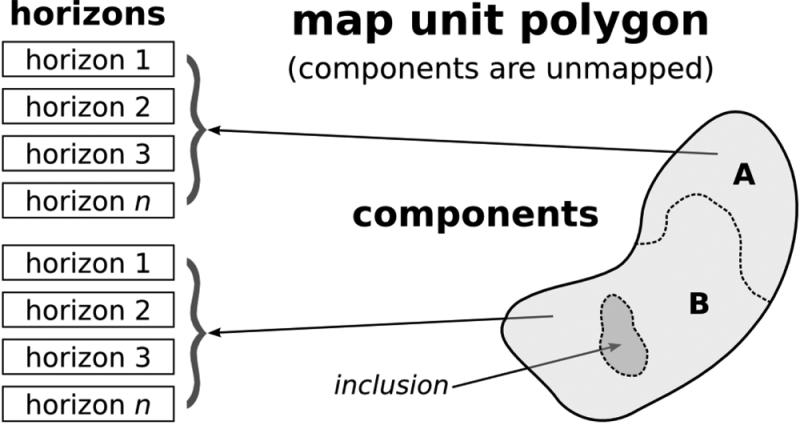
\includegraphics[width=0.5\textwidth]{./img/ssurgo_data_structure_schematic.jpeg}
	\caption[Schematic diagram of SSURGO data structure]{Schematic diagram of SSURGO data structure \cite{gatzke_aggregation_2011}}.
	\label{fig:ssurgo_schematic}
\end{figure}

We chose to use the gSSURGO distribution of SSURGO. gSSURGO is a form of the SSURGO database that is packaged in a more
convenient form for GIS users. The tabular data representing the components and
horizons were joined together so that each component had the data required for
the SWAT model; these properties were hydrologic soil group (HSG), albedo,
horizon depths, bulk density, available water capacity, organic matter,
saturated conductivity, total percentage of clay/silt/sand, USLE K factor,
electrical conductivity, calcium carbonate concentrations, pH (1 to 1 in water),
and coarse fragment percentage. Of these, the hydrologic soil group and albedo
were stored at the component level, while all other properties were stored at
the horizon level. For all these properties, the representative value given by
SSURGO was used. For more information about these parameters see the SSURGO
metadata\footnote{\url{http://www.nrcs.usda.gov/wps/portal/nrcs/detail/soils/survey/?cid=nrcs142p2_053631}}.

HRU definition in a SWAT model is a balance of incorporating the most important
pieces of information without overloading it with redundant or insignificant
information---a modeler should represent every process that controls the system,
however an overloaded model requires more computational resources, which may not
be feasible to acquire. To reduce the number of HRUs in the model, we aggregated
soils together based on similarity of several key properties that impact the
hydrologic cycle. This was a two step process: first, components within map
units were aggregated
together\footnote{\url{https://github.com/dnrwaterqualitymodeling/wisconsinRiverTMDL/blob/master/soils/step1_aggregate_gSSURGO.R}},
and second, map units were aggregated together based on
similarity\footnote{\url{https://github.com/dnrwaterqualitymodeling/wisconsinRiverTMDL/blob/master/soils/step2_aggregate_gSSURGO.R}}.

Several changes were made to the dataset before aggregation, in order to
facilitate processing. Soil organic carbon content is required by SWAT, but is
given by SSURGO as soil organic matter. The organic matter (percent) value given in SSURGO
was converted to percent organic carbon by multiplying by 50\% which is the generally accepted average carbon content of soil organic matter \citep{brady_elements_2004}. The HSG is
denoted as a letter in SSURGO, either A through D, or if the soil has different
characteristics when drained, as two letters, A/D, B/D or C/D, the latter of
which is the natural state of the soil if not artificially drained (e.g.,
through tiling or ditching) while the former is if the soil is drained. In order
to average the different components it was necessary to convert these letters
into numbers; groups A through D were converted to 1 through 4 to correspond
with increasingly wetter drainage conditions. Once a number was obtained for the
HSG, it was treated as any other soil property in the aggregation process and
then rounded to the nearest integer and converted in the same manner to a letter
once the aggregation was finished. For those components with dual HSGs, we
assumed that if half of the area in the map unit was agriculture it was drained
and the first HSG taken; conversely, if the landuse was not majority agriculture
then it was assumed to not be drained and the ``D'' designation was chosen.

The first aggregation step was to aggregate components by map unit to conform to
the SWAT soils data structure. The data structure for soils in SWAT does not
directly conform to SSURGO data structure, mainly that there is no analog to the
SSURGO \textit{component} level in SWAT---in other words, soils in SWAT cannot
be subdivided, see figure \ref{fig:component_schematic}. We aggregated components by computing
component-weighted averages of each soil property for any given depth of soil from the soil surface to the average depth\cite{gatzke_aggregation_2011, beaudette_algorithms_2013}.
These averages were computed using the \texttt{slab} function in the \texttt{aqp} package in R \cite{beaudette_algorithms_2013}. We
used this algorithm to apply a depth weighted average to each horizon, while
also weighting the percent composition of each component. This achieved a robust
average of the soil properties for each horizon, while also accounting for
differing compositions of each component. The depth and number of horizons of
the aggregated soil profile produced by this algorithm must be specified before
processing. The depth was calculated by using the weighted mean of the depths of
the components, with the weights equal to the percent composition of each
component. As the number of horizons was not seen to matter as much as the
maximum depth, an arbitrary number of five horizons was chosen for the
aggregation algorithm.

\begin{figure}[h]
  \centering
    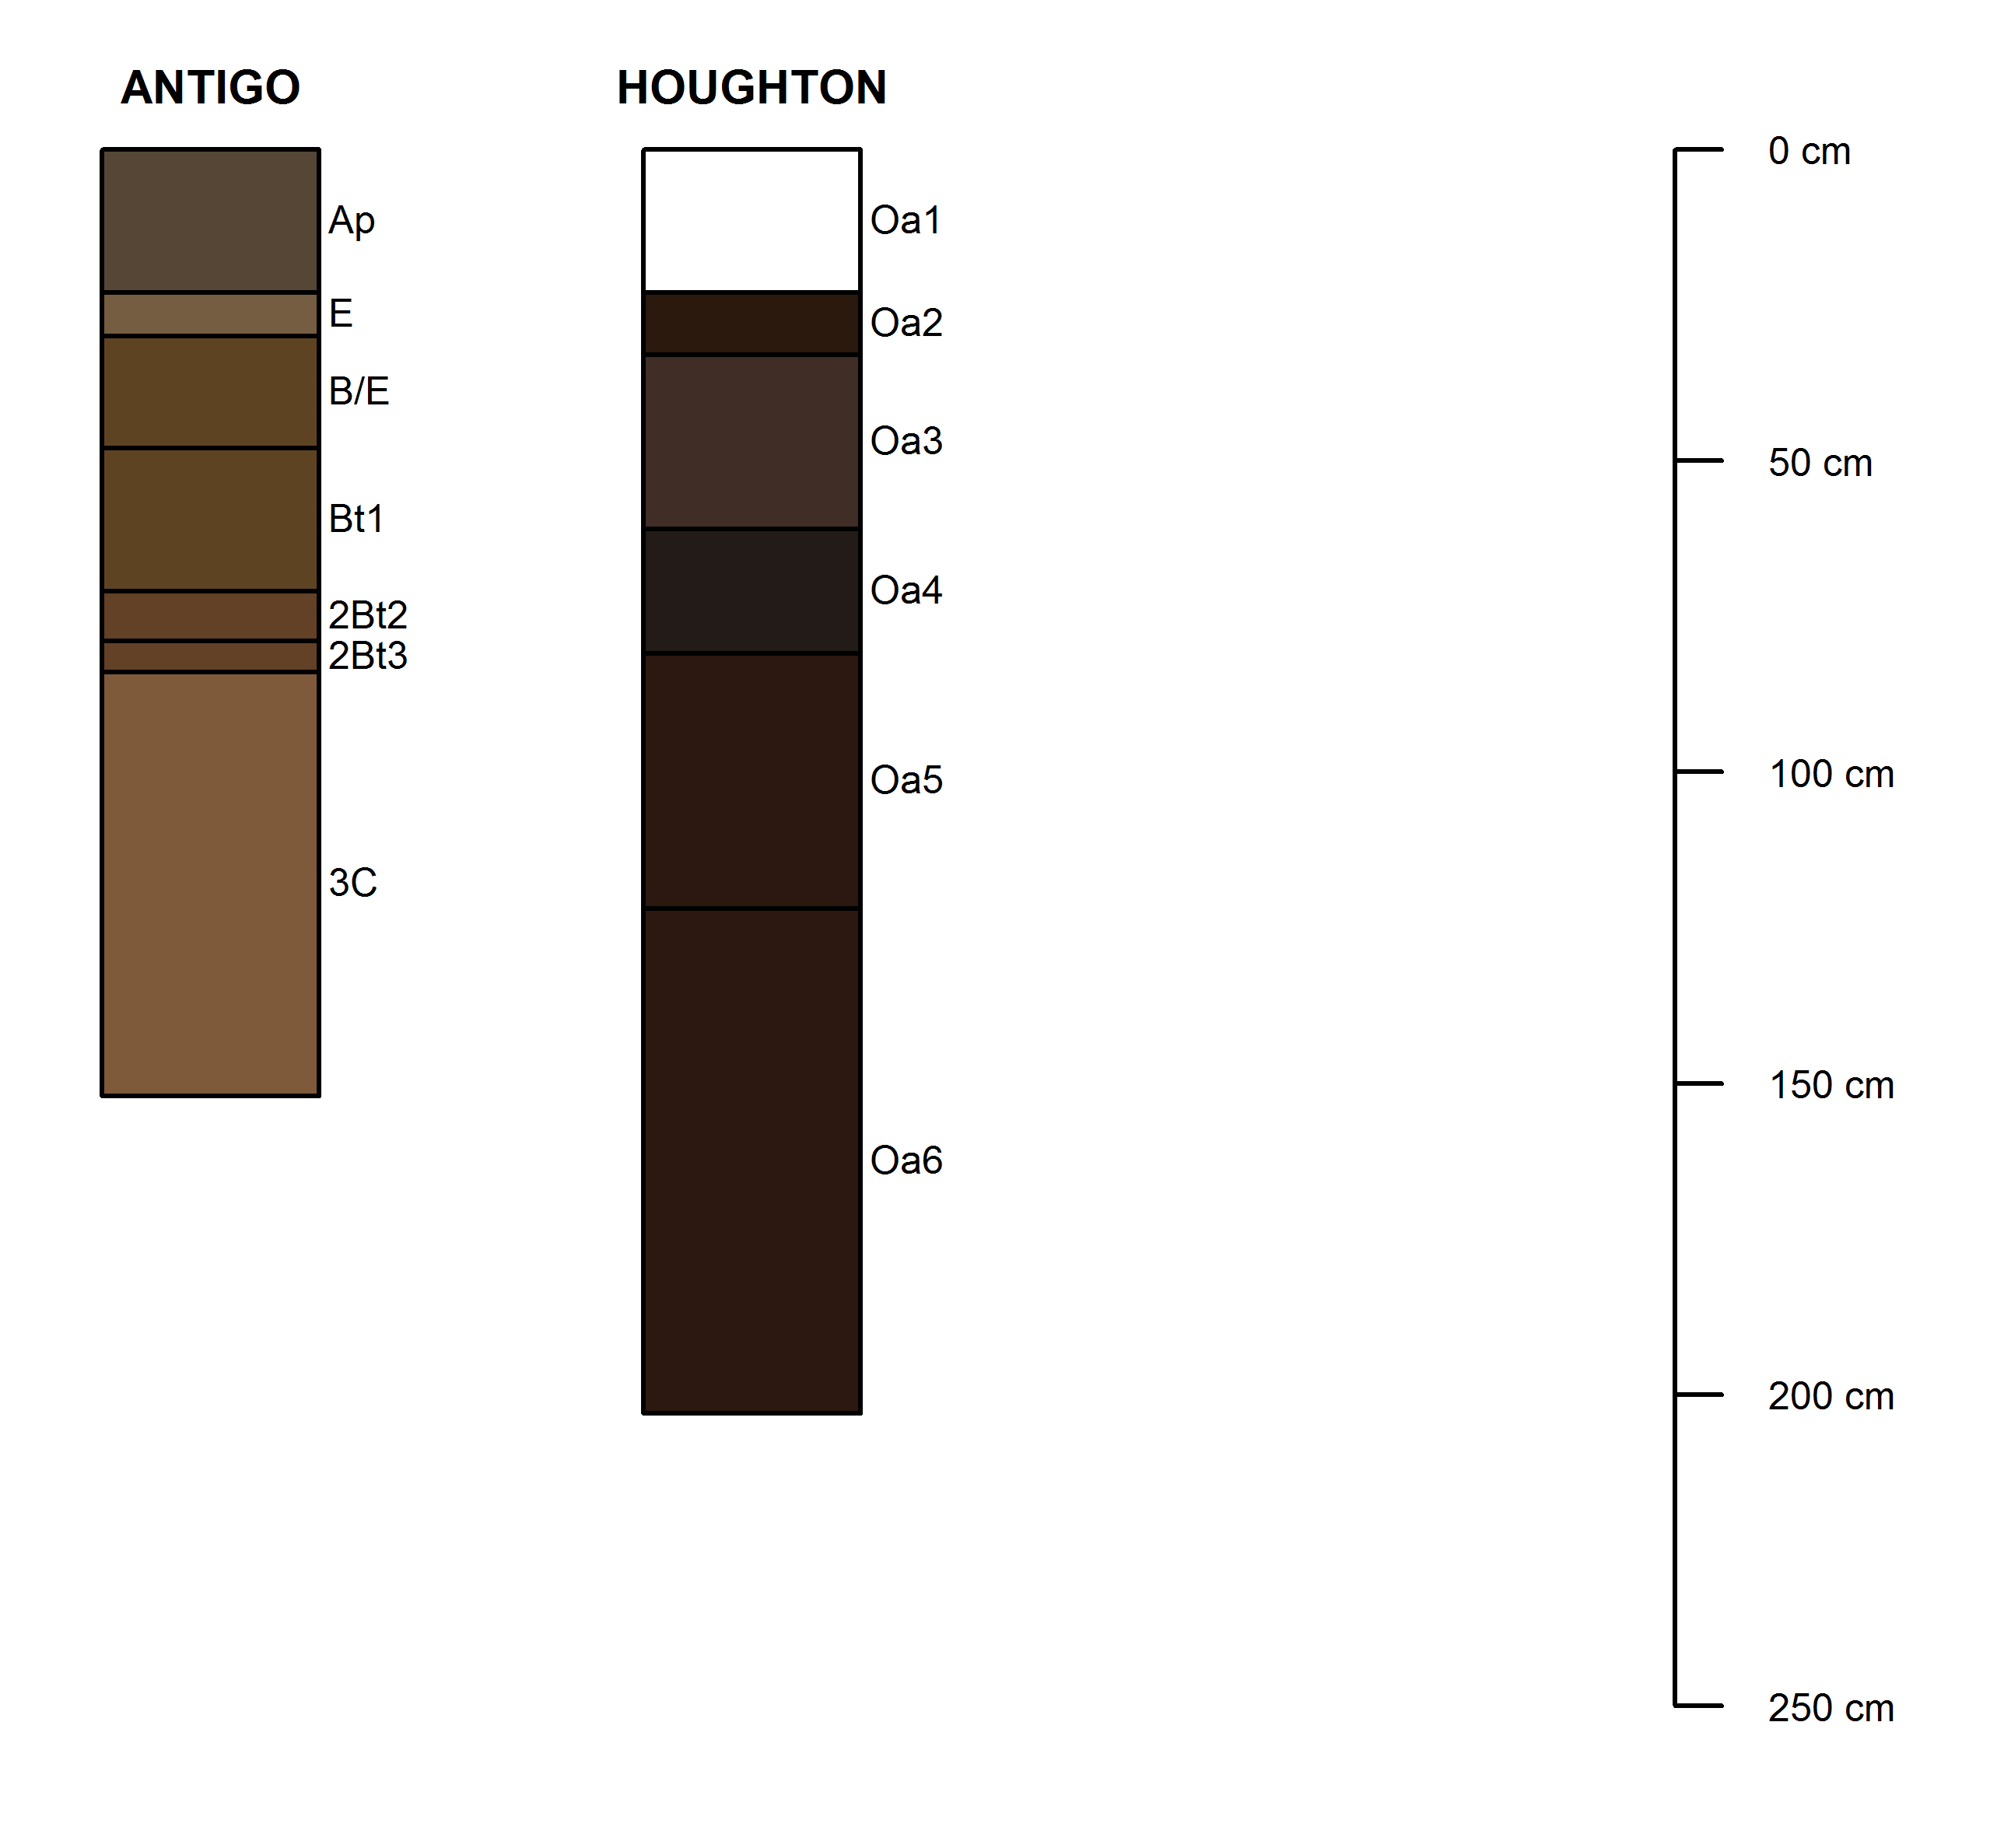
\includegraphics[width=0.5\textwidth]{./img/component_schematic.png}
	\caption[Schematic diagram of SSURGO map unit]{Schematic diagram of SSURGO map unit. Antigo and Houghton are each components within the map unit. Within each map unit are varying numbers of components with varying horizon depths (e.g., Ap and O1 are the surface horizons for Antigo and Houghton respectively. Components were aggregated to map units by averaging soil properties (e.g., percent sand) horizontally across horizons.}
	\label{fig:component_schematic}
\end{figure}

Using the above aggregation method 48,585 individual soil components were
aggregated to 1,603 map units. Because the HRU used in
SWAT is derived using unique combinations of land use, slope and soil types,
this number of soil map units is still too many for efficient computation  and so
the second step of the soils data configuration was necessary to further reduce
the number of soil types. %\textbf{[More justification necessary?]}

Other researchers have aggregated soil types by their taxonomic class
\citep{gatzke_aggregation_2011} but Soil Taxonomy, the soil classification
system of the US, classifies largely based on soil morphology and not
necessarily on SWAT relevant properties. We decided that the most relevant soils
information to SWAT is hydrology data, specifically the HSG, which has a large impact on the curve number calculation. With this
consideration, aggregation was based around (and so preserved) the HSG of the
map unit. Groups of the same HSG were divided into smaller groups, hereafter
known as clusters, of homogeneous soil properties, using a clustering algorithm.
The map units within each of these clusters were then averaged together to create
an average profile for that homogeneous set of soils. These averages were then
used as the soil types for the HRU definitions and the SWAT modeling.

Each map unit was placed into one of four groups according to its hydrologic soil
group, A, B, C or D. To subdivide these groups further, a clustering algorithm
was used to objectively and robustly create clusters of map units with
homogeneous soil properties. For this purpose we used Gaussian mixture models to
assign map units to clusters. The mixture model algorithm we used was implemented within the
\texttt{Mclust} function in the mclust package \citep{fraley_mclust_2012} in R.
A mixture model is a probabilistic model for representing the presence of
subpopulations within an overall population. In our case, the overall population
would be the group of map units of like hydrologic soil groups (say all map units
with an HSG of A), while the (unknown) subpopulations are the clusters of
map units with similar distributions of soil properties (such as a cluster of
sandier soils, shallow soils or slow saturated conductivity). Using the default
settings of the function, the algorithm clustered all of the A HSG map units into
6 clusters, and all of the other HSG classes into 9 clusters.

Each of the 1603 map units had data regarding the soil property values at each
horizon. In this format it was thought that profile depth would have undue influence over the clustering algorithm, that is deep soils would cluster together and shallow soils cluster together regardless of the nature of the other properites, causing clusters to be entirely governed by
depth. To remedy this issue, depth weighted averages of the horizons were taken
to derive one value per soil property for each map unit; essentially collapsing
the soil profile down to one aggregate horizon. Profile depth was still
considered in the clustering algorithm by keeping the profile depth as a
property and so in this way it is represented but does not dominate the clustering
algorithm.

Not every map unit was included in the clustering procedure. Several of the soil property fields of the SSURGO dataset were not populated or commonly had ``no data'' values, these properties were not used in the
clustering process so the spurious zeros would not influence the algorithm. These properties were coarse fragments, calcium carbonate, and electrical conductivity. Albedo and pH were also excluded from the clustering algorithm. Mapunits that had no HSG designation were not included, nor were map units that did not have information on the soil properties of the horizons. Examining these excluded map units revealed that they were generally disturbed landscapes or those without a significant soil layer such as pits, landfills, urban or made land, rock outcrops, and water. These miscellaneous map units were all grouped together as one cluster with the exception of water, which we did not use in the cluster analysis.

The same soil profile aggregation algorithm \citep{beaudette_algorithms_2013}
used to aggregate several components together in the first step was used to combine the soil profiles of a cluster into one
composite soil profile. In this implementation each map unit was given equal
weight in the aggregation algorithm. Those map units designated as miscellaneous
were aggregated into one soil profile as the other clusters were, while the
water map units were not aggregated. The miscellaneous grouping was assigned an
HSG by converting the letter designation into an ordinal
integer (that is A, B, C, D to 1, 2, 3, 4) and the average was taken, rounded to
the nearest integer, and converted back to a letter, which happened to be B. Following SWAT convention, the water units
were given an HSG of D, and assigned an albedo of 0.23, and a saturated conductivity
of 600.

A total of 35 soil classes were distilled from this process. An example of the properties of can be seen in \ref{table:soil_prop} and the number of map units in each cluster can be found in 	\begin{table}[h!]
	\caption{Number of mapunits in each cluster.}
	\centering
		\begin{tabular}{c c c c c}
			\hline 
			Cluster Number	 & 	A	 & 	B	 & 	C	 & 	D \\
			\hline \hline
			1 & 33	& 79	& 51	& 36  \\
			2 & 72	& 50	& 42	& 17  \\
			3 & 57	& 152	& 18	& 15  \\
			4 & 45	& 41	& 11	& 15  \\
			5 & 54	& 284	& 36	& 9   \\
			6 & 32	& 120	& 16	& 12  \\
			7 & NA	& 68	& 12	& 6   \\
			8 & NA	& 70	& 25	& 11  \\
			9 & NA	& NA  	& 6 	& 10  \\
			\hline		
		\end{tabular}
		
		\label{table:soil_clust}
	\end{table}	
	


.

The hydrologic soil groups and the clusters within these groups are displayed in figure \ref{fig:soil_boxplots}. This figure shows the relative variability for each soil property for each cluster.
\begin{table}[h!]
	\centering
		\begin{tabular}{l c c c c c c c}
			Class	 & 	Total Depth	 & 	$D_B$	 & 	AWC	 & 	$K_{sat}$	 & 	C \%	 & 	Clay \%	 & 	Sand \% \\[0.25ex]
			\hline \hline
			A1	 & 	1525.30	 & 	0.00	 & 	0.46	 & 	125.37	 & 	37.25	 & 	0.00	 & 	0.00  \\
			A2	 & 	1520.55	 & 	1.58	 & 	0.10	 & 	185.52	 & 	0.61	 & 	6.25	 & 	83.37 \\
			A3	 & 	1528.08	 & 	1.63	 & 	0.09	 & 	267.17	 & 	0.61	 & 	3.77	 & 	84.64 \\
			A4	 & 	1454.86	 & 	1.30	 & 	0.27	 & 	185.29	 & 	17.88	 & 	2.21	 & 	44.51 \\
			A5	 & 	1805.87	 & 	1.58	 & 	0.14	 & 	243.14	 & 	4.24	 & 	4.59	 & 	71.70 \\
			A6	 & 	1522.91	 & 	1.65	 & 	0.07	 & 	271.49	 & 	0.47	 & 	3.49	 & 	93.86 \\
			B1	 & 	1520.00	 & 	1.55	 & 	0.18	 & 	50.53	 & 	0.94	 & 	12.48	 & 	47.51 \\
			B2	 & 	1537.39	 & 	1.50	 & 	0.22	 & 	27.17	 & 	0.93	 & 	19.04	 & 	12.22 \\
			B3	 & 	1520.09	 & 	1.59	 & 	0.13	 & 	94.29	 & 	0.68	 & 	8.55	 & 	70.05 \\
			B4	 & 	1544.18	 & 	1.58	 & 	0.12	 & 	195.90	 & 	2.00	 & 	6.71	 & 	75.42 \\
			B5	 & 	1522.91	 & 	1.52	 & 	0.20	 & 	42.73	 & 	1.07	 & 	13.44	 & 	38.50 \\
			B6	 & 	1577.51	 & 	1.45	 & 	0.20	 & 	50.08	 & 	5.19	 & 	11.79	 & 	36.19 \\
			B7	 & 	1533.33	 & 	1.57	 & 	0.15	 & 	40.36	 & 	1.61	 & 	6.84	 & 	62.35 \\
			B8	 & 	2002.61	 & 	1.51	 & 	0.22	 & 	27.73	 & 	0.74	 & 	18.15	 & 	12.74 \\
			B9	 & 	1521.05	 & 	1.37	 & 	0.22	 & 	27.11	 & 	1.32	 & 	20.30	 & 	9.76 \\
			C1	 & 	1521.39	 & 	1.55	 & 	0.20	 & 	27.66	 & 	0.90	 & 	12.32	 & 	29.21 \\
			C2	 & 	1520.00	 & 	1.56	 & 	0.18	 & 	36.30	 & 	0.92	 & 	11.11	 & 	49.20 \\
			C3	 & 	1710.42	 & 	1.60	 & 	0.18	 & 	24.39	 & 	0.74	 & 	20.46	 & 	27.03 \\
			C4	 & 	1520.44	 & 	1.58	 & 	0.14	 & 	52.02	 & 	0.97	 & 	10.45	 & 	62.91 \\
			C5	 & 	1731.63	 & 	1.51	 & 	0.19	 & 	54.78	 & 	3.14	 & 	9.04	 & 	41.07 \\
			C6	 & 	1526.38	 & 	1.49	 & 	0.22	 & 	27.46	 & 	1.23	 & 	16.13	 & 	14.31 \\
			C7	 & 	1529.74	 & 	1.63	 & 	0.13	 & 	274.05	 & 	2.88	 & 	6.00	 & 	76.92 \\
			C8	 & 	1583.62	 & 	1.49	 & 	0.20	 & 	26.05	 & 	1.04	 & 	20.47	 & 	23.93 \\
			C9	 & 	2072.00	 & 	1.41	 & 	0.18	 & 	64.26	 & 	4.88	 & 	5.00	 & 	55.33 \\
			D1	 & 	1520.21	 & 	1.52	 & 	0.18	 & 	69.54	 & 	2.53	 & 	13.67	 & 	46.29 \\
			D2	 & 	1521.23	 & 	0.95	 & 	0.40	 & 	68.93	 & 	34.45	 & 	1.64	 & 	5.50 \\
			D3	 & 	760.00	 & 	1.36	 & 	0.19	 & 	29.40	 & 	1.48	 & 	17.53	 & 	34.80 \\
			D4	 & 	1520.00	 & 	1.61	 & 	0.17	 & 	52.55	 & 	0.84	 & 	14.04	 & 	51.78 \\
			D5	 & 	1813.33	 & 	1.66	 & 	0.18	 & 	16.90	 & 	2.36	 & 	28.73	 & 	20.09 \\
			D6	 & 	1552.68	 & 	1.43	 & 	0.26	 & 	215.82	 & 	15.40	 & 	2.66	 & 	41.92 \\
			D7	 & 	1520.00	 & 	0.00	 & 	0.40	 & 	66.00	 & 	38.75	 & 	0.00	 & 	0.00 \\
			D8	 & 	1520.00	 & 	1.39	 & 	0.24	 & 	27.71	 & 	4.35	 & 	22.94	 & 	8.00 \\
			D9	 & 	1796.86	 & 	1.25	 & 	0.20	 & 	50.65	 & 	5.10	 & 	7.76	 & 	39.68 \\
			W	 & 	25.00	 & 	0.00	 & 	0.00	 & 	600.00	 & 	0.00	 & 	0.00	 & 	0.00 \\
			X	 & 	416.77	 & 	1.78	 & 	0.02	 & 	157.56	 & 	0.49	 & 	5.86	 & 	78.24 \\
			\hline		
		\end{tabular}
		\caption{Soil property data for the first horizon of each class. Total depth is the depth of entire profile, not just the horizon. Abbreviations: $D_B$ is bulk density, AWC is available water capacity, $K_{sat}$ is saturated conductivity, C \% is carbon percentage, clay \% is percentage of clay-size particles, and sand \% is precentage of sand size particles.}
		\label{table:soil_prop}
	\end{table}	
	
	 
\begin{figure}[H]
  \centering
    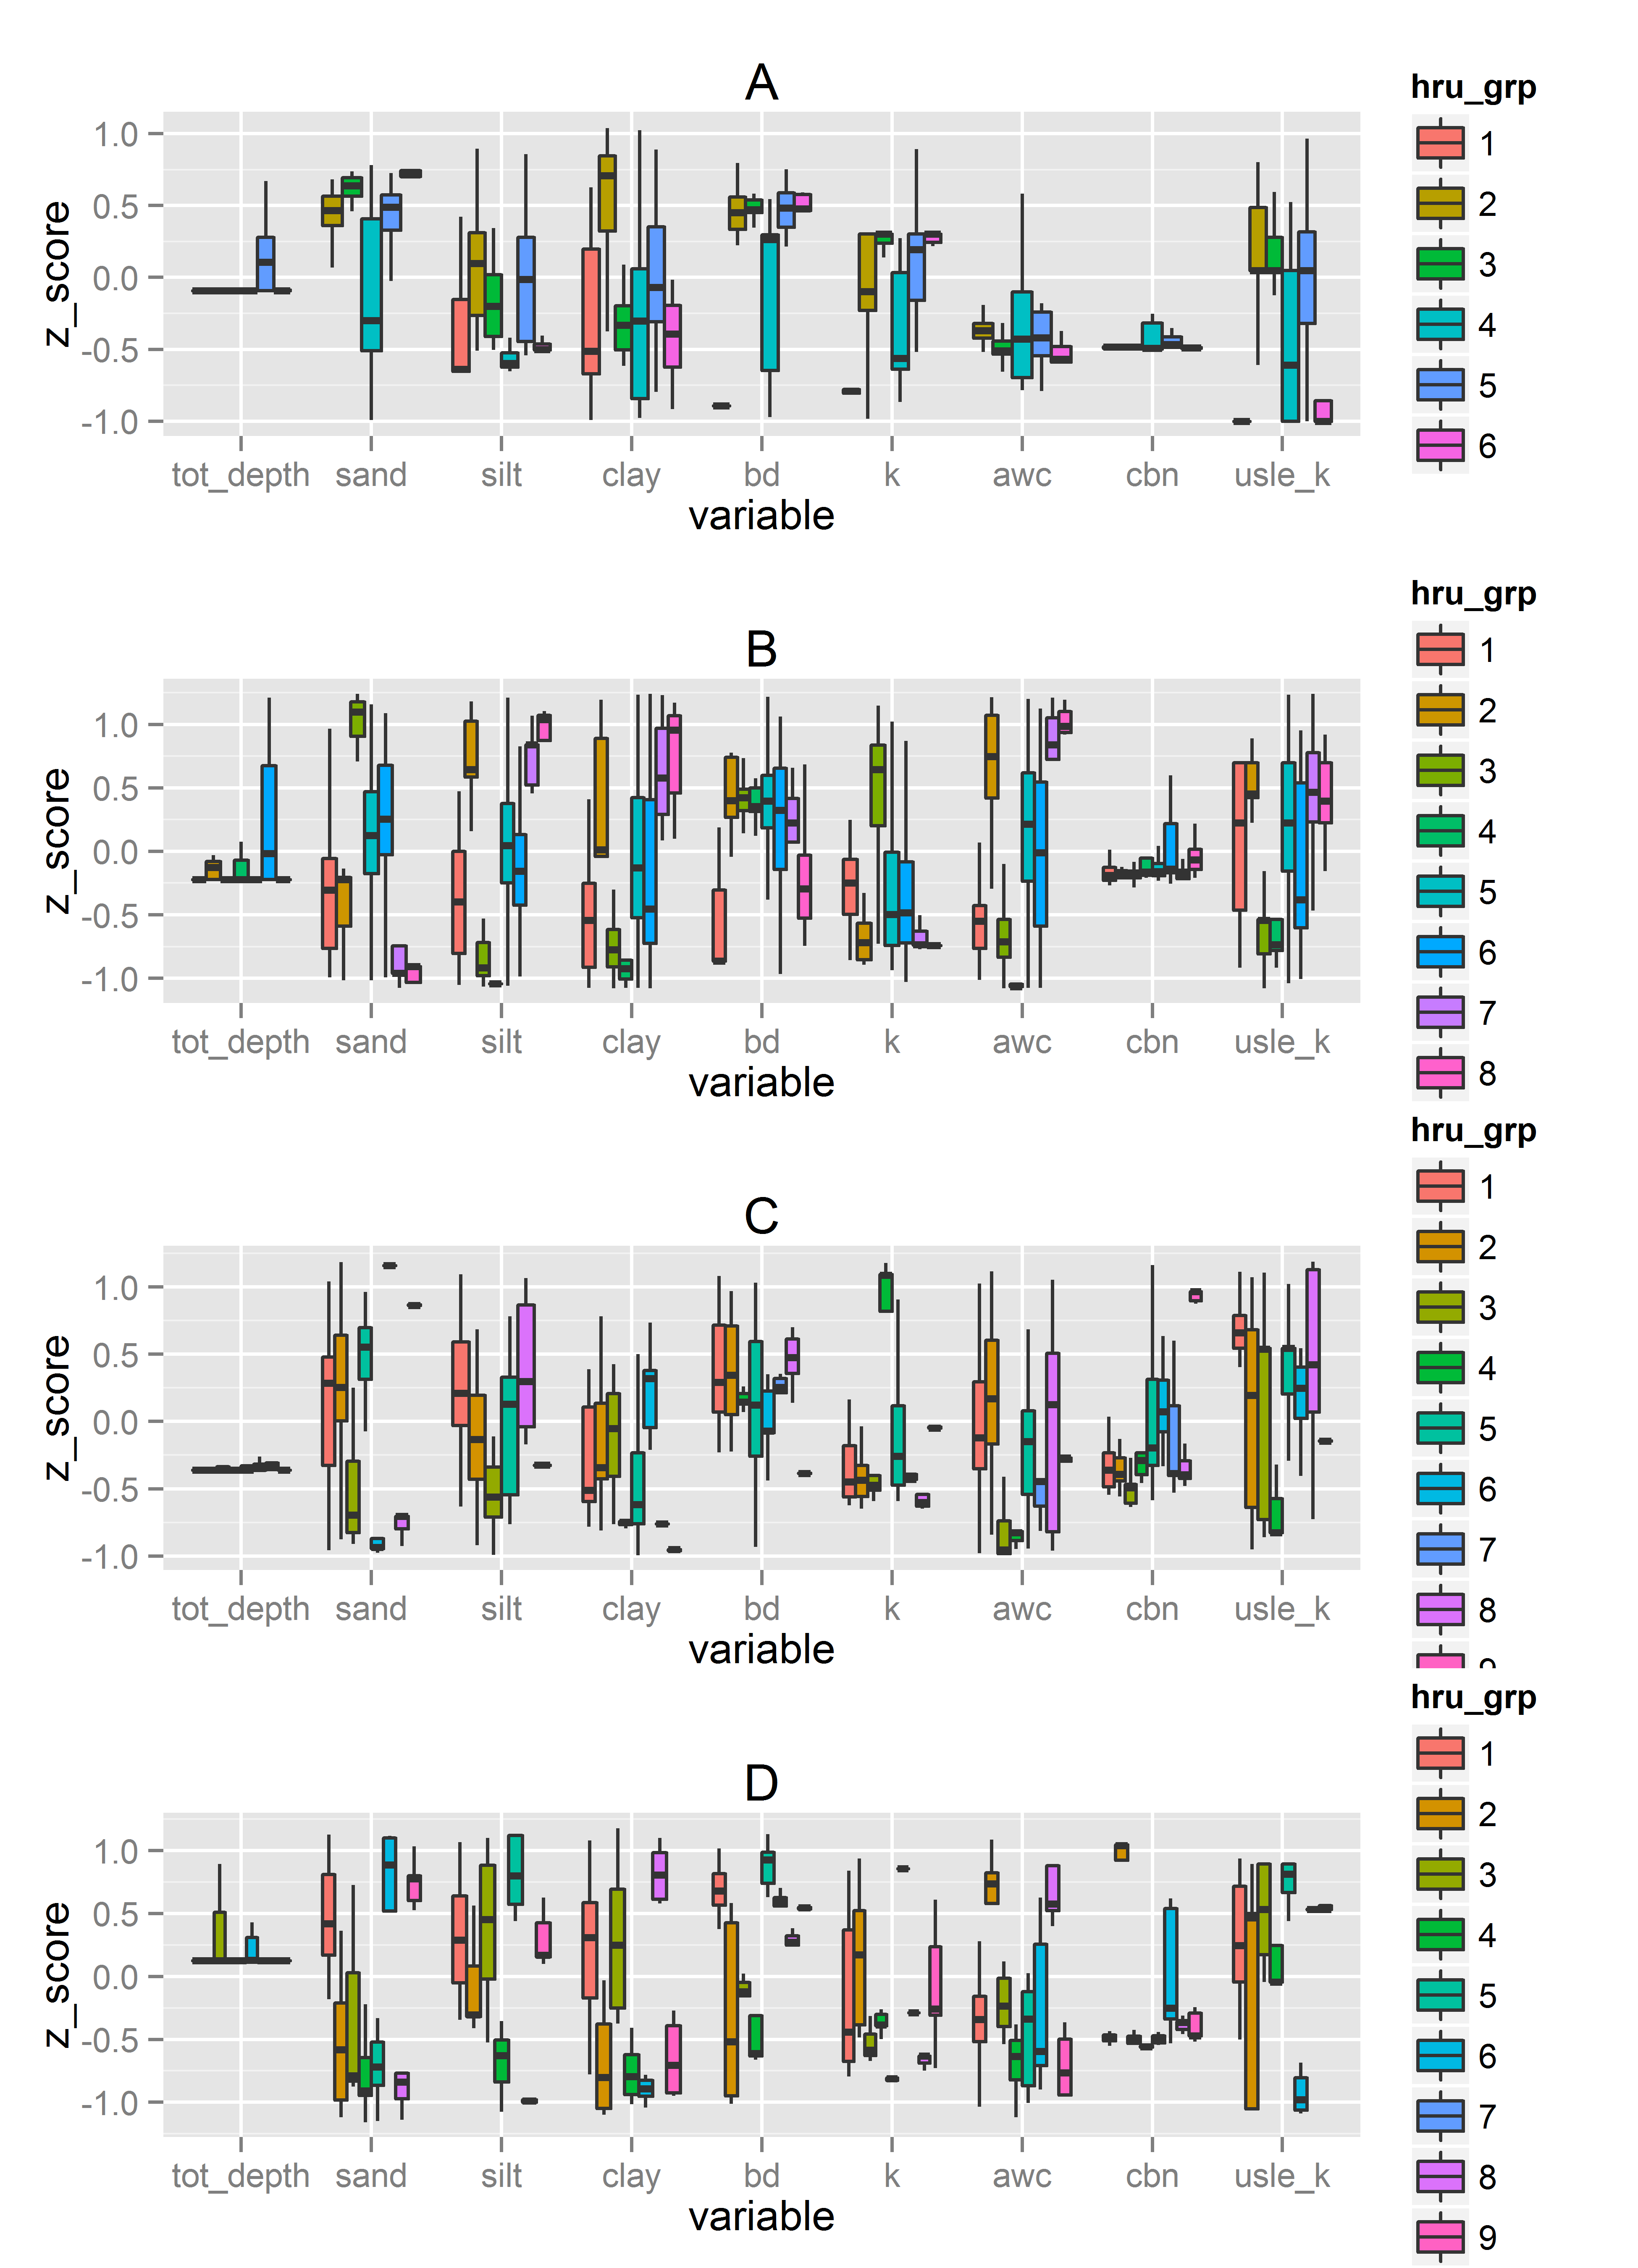
\includegraphics[width=\textwidth]{./img/cluster_variability.png}
	\caption[Boxplots showing the variability of soil properties]{Boxplots showing the variability of soil properties within the final set of soil clusters. The letter above each plot denotes hydrologic soil group (HSG). Each color represents a cluster of map units. The Z score for each soil property is reported as $Z = X - \mu / \sigma$ where $X$ is the value of the soil property, $\mu$ and $\sigma$ are the population mean and standard deviation of a soil property. Outliers were excluded. The x-axis shows soil properties where tot\_depth is the soil depth, sand/silt/clay are the percent composition of each texture class, bd is bulk density, k is saturated conductivity, awc is available water capacity, cbn is organic carbon concentration, and usle\_k is soil erodibility.}
	\label{fig:soil_boxplots}
\end{figure}

Soil Phosphorus concentrations were obtained through the University of Wisconsin
Soil Testing Laboratory \footnote{\url{http://uwlab.soils.wisc.edu/}}. Soil
phosphorus concentrations were aggregated by county by the soil laboratory for
each year from 1974 to the present. We chose the annual average soil
concentration nearest the beginning of the model spin-up period, 1995, to
establish prior concentrations. Subbasin-level soil phosphorus concentrations
were estimated by calculating an area-weighted average of intersecting counties
within a subbasin.
The soil testing laboratory receives almost exclusively agricultural soils so to reflect this bias in the soil phosphorus data, only agricultural HRUs were given the subbasin average concentration, while the non-agricultural HRUs were given SWAT's default concentration (5 mg P/Kg). This default concentration is assumed to equilibrate over the 6-year model spin-up period. 
Soluble phosphorus
concentrations were estimated as half of the reported phosphorus using the
Bray-1 method measured with a spectrophotometer \citep{vadas_validating_2010}.
Organic phosphorus concentrations were estimated by assuming that phosphorus
constitutes 0.85\% of organic material measured by loss of weight upon ignition
(correspondence with Phillip Barak, needs citation). Soil phosphorus estimates are not included in the SWAT model provided---they will be included during the phosphorus calibration phase.
